\documentclass{beamer}

\usepackage[T1]{fontenc} 
\usepackage[latin1]{inputenc}
%% \usepackage[frenchb]{babel}

\usetheme{Warsaw}

% Supprimer les icones de navigation (pour les transparents)
\setbeamertemplate{navigation symbols}{}

\title[Presentation for Institut Pasteur]{Presentation at Institut Pasteur~\\Proteomic BioInformatic Position}
\author{Gabriel Chandesris}
%% \institute{ --- }
\institute{ 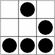
\includegraphics[height=0.5cm]{img/logo_glider.png} }
%% \logo{ 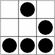
\includegraphics[height=2.5cm]{img/logo_glider.png} }
\date{September 3rd, 2020} %% \date{\today}

\begin{document}

\begin{frame}
	\titlepage
\end{frame}

\begin{frame}
	\frametitle{Table Of Content}
	\small \tableofcontents[hideallsubsections]
\end{frame} 

\def\titleSectionCurriculumPart{Curriculum Part}
\section{\titleSectionCurriculumPart }
\begin{frame}
	\frametitle{\titleSectionCurriculumPart }
	\tableofcontents[sections=1,currentsection,subsectionstyle=show/shaded/hide]
\end{frame} 

\def\titleSubSectionCurriculumPartOne{Starting points}
\subsection{ \titleSubSectionCurriculumPartOne }
\begin{frame}
	\frametitle{ \titleSubSectionCurriculumPartOne }
	\begin{columns}[T]
	\begin{column}[T]{6.0cm}
		\begin{block}{What I Wanted to do}
			\begin{itemize}
				\item Major interest for Computers and related Tools ; 
				\item Interest for Science and Biology ; 
				\item Experimentations in both domains ; 
				\item[] 
				\item Curiosity ! (and some ideas)
			\end{itemize}
		\end{block}
	\end{column}
	\begin{column}[T]{5.0cm}
		\begin{block}{Diplomas (``French Intitul{\'e}s'') }
			\begin{itemize}
				\item \textbf{2000} Baccalaur{\'e}at Scientifique Sp{\'e}cialit{\'e} Sciences de la Vie et de la Terre ; 
				\item \textbf{2003} BTS Biochimiste ; ~\\
				Training: ``\emph{Diagnostic de l'h{\'e}mochromatose g{\'e}n{\'e}tique par biologie mol{\'e}culaire -- Validation d'une technique automatis{\'e}e}''
				%% \item ... \emph{the following in next slides !}
			\end{itemize}
		\end{block}
	\end{column}
	\end{columns}
\end{frame} 

\def\titleSubSectionCurriculumPartTwo{Continuation (working and studying on same time)}
\subsection{ \titleSubSectionCurriculumPartTwo }
\begin{frame}
	\frametitle{ \titleSubSectionCurriculumPartTwo }
	\begin{itemize}
		\item Working as Lab Technicien / Engineer (medical analysis) ; 
		\item Night class in \emph{Conservatoire National des Arts et M{\'e}tiers} ; 
		\item Certification (2005) then Licence (2007) in BioInformatics 
		(training at Sanofi R\&D SCDM : a data integration module)
		\item[]  
		\item \textbf{2009} Master of BioInformatics at Evry (near Genopole)
		\begin{itemize}
			\item Train on Year 1 : IBISC CNRS Lab at Evry ("Industrialisation d'un logiciel pour la pr{\'e}diction de structures secondaires d'ARN non codants")
			\item Train on Year 2 : Dassault Syst{\`e}mes ("F{\'e}d{\'e}ration de bases de donn{\'e}es en sciences de la vie -- Conception et mise en place d'un prototype dans ENOVIA V6")
		\end{itemize}
	\end{itemize}
\end{frame}

\begin{frame}
	\frametitle{ Train on Master Year 1 : IBISC CNRS Lab at Evry }
	
	\texttt{ \small "Industrialisation d'un logiciel pour la pr{\'e}diction de structures secondaires d'ARN non codants"}
	
	\begin{columns}[T]
	\begin{column}[T]{6.5cm}
	
		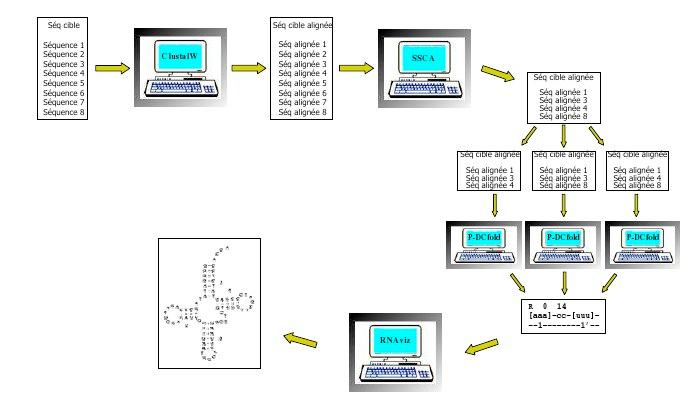
\includegraphics[width=6.5cm]{img/illustrationStageIBISC.png} 
	
	\end{column}
	\begin{column}[T]{6.0cm}
	
		\begin{itemize}
			\item Analyze of Biology Context (Studies of RNA, analyse and predict structures) ; 
			\item Approach is use of different algorithms (ClustalW, SSCA, PDCFold)
			\item Analyze of Existing Software (a JAVA Stand-Alone Application), Documentation \& Reverse Engineering ; 
			\item Adaptation to Web (in an Apache Tomcat Server) ; 
			\item ... 
		\end{itemize}
		
	\end{column}
	\end{columns}
	
\end{frame}

\begin{frame}
	\frametitle{ Train on Year 2 : Dassault Syst{\`e}mes }
	
	\texttt{ \small "F{\'e}d{\'e}ration de bases de donn{\'e}es en sciences de la vie -- Conception et mise en place d'un prototype dans ENOVIA V6"}
	
	\begin{columns}[T]
	\begin{column}[T]{6.0cm}
	
		\begin{itemize}
			\item DataBases : InterPro, UniprotKB, PDB ; 
			\item Documentation and bibliography, 
			\item Review, comparisons (mediation, data warehouse) and limitations, 
			\item Data Mapping ; 
			\item Prototyping ; 
			\item ... 
		\end{itemize}
	
	\end{column}
	\begin{column}[T]{6.5cm}
	
		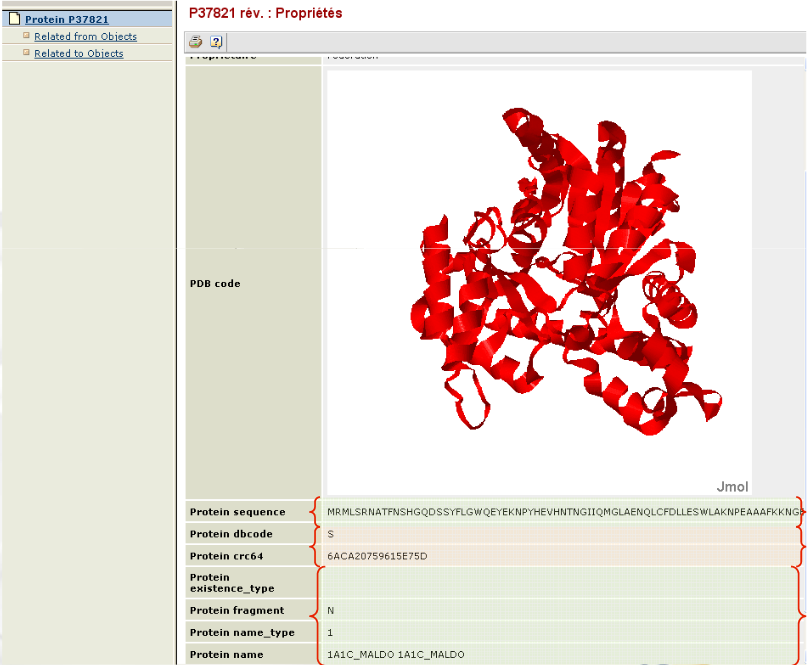
\includegraphics[width=6.5cm]{img/illustrationStage3DS.png} 
	
	\end{column}
	\end{columns}
	
\end{frame}

\def\titleSubSectionCurriculumPartThree{Data treatment, BioInformatics, Software Dev, Trainer...}
\subsection{ \titleSubSectionCurriculumPartThree }
\begin{frame}
	\frametitle{ \titleSubSectionCurriculumPartThree }
	\begin{itemize}
		\item EDD (2009-2010) : working on building a complete framework (in Perl) of Data Treatment (from tabular files and XML to a Postgre Relational DataBase, SQL) ;
		\item SoBioS then Dassault Syst{\`e}mes (BIOVIA brand) ; European BioIntelligence project, 2010 to 2018 :
		\begin{itemize}
			\item Prototyping, modeling, documentations, presentations...
			\item Regular meeting with Pharma (Ipsen, Servier, Sanofi)
		\end{itemize}
		\item Consultant at OXiane (2018-2020) and working with JAVA tools and frameworks : 
		\begin{itemize}
			\item Maintaining and Developping Software for client ; 
			\item Starting internal train for Apache Kafka framework (performant Messaging and Log Service). 
		\end{itemize} 
	\end{itemize}
\end{frame} 


\def\titleSectionPositionPart{Position Part}
\section{\titleSectionPositionPart }
\begin{frame}
	\frametitle{\titleSectionPositionPart }
	\tableofcontents[sections=2,currentsection,subsectionstyle=show/shaded/hide]
\end{frame} 

\def\titleSubSectionPositionPartOne{What I come with : Experiences in previous positions !}
\subsection{ \titleSubSectionPositionPartOne }
\begin{frame}
	\frametitle{ \titleSubSectionPositionPartOne }
	\begin{itemize}
		\item I worked in Private Companies (mostly) and some Public ; 
		\item Knowledge of working habits and working methods in these domains (precisions on next slide) ;  
		\item[]
		\item Biology, Biochemistry, Immunology... (technical positions)
		\item Computer Engineering, especially software development (scripting, OOP, Delivery and Integration, Design Patterns) ; 
		\item BioInformatics : databases and data integration, data treatment (algorithms)... 
		\item[] 
		\item \emph{Computer and software development as TOOLS for Biology and BioInformatics !}
	\end{itemize}
\end{frame} 

\def\titleSubSectionPositionPartTwo{What I come with ! Working methods ?!}
\subsection{ \titleSubSectionPositionPartTwo }
\begin{frame}
	\frametitle{ \titleSubSectionPositionPartTwo }
	\begin{itemize}
		\item V-Cycle : force the formalism and documentation and tests, mid- and long-term projects ; 
		\item Agile / Scrum and eXtreme Programming (XP) : iteration and 'continuous' delivery ; 
		\item Tests, Prototyping and Industrialisation
		\item Documentation : 'Office' and similar, \LaTeX , MarkDown, Wiki, Source Code (DOxygen / JavaDoc)...
		\item xUnit, Mockito, MockNeat : Unit Tests, Integration, Data ; 
	\end{itemize}
\end{frame} 

\def\titleSubSectionPositionPartThree{What I come with ! Technologies and other elements !}
\subsection{ \titleSubSectionPositionPartThree }
\begin{frame}
	\frametitle{ \titleSubSectionPositionPartThree }
	\begin{itemize}
		\item Programming languages and their libraries / frameworks : Java, Perl, Shell (Bash), some knowledge of Python and C/C++
		\item Data manipulation, Extraction and Treatment, in different file formats and databases : tabular, CSV, XML... And some from BioInformatics Tools (FASTA, ClustalW...) !
		\item ``\emph{Software CraftmanShip}'' 
		\item Some tools : SourceCode / Project versionning (SVN and GIT), IDEs (Eclipse and similar), OS (preference for Unix / Linux but MacOS X and Windows exists !)... 
		\item Trainer / Mentor : always seeking for examples to make a better learning and transmission of knowledge. 
	\end{itemize}
\end{frame} 

\def\titleSectionQuestionPart{Questions ?!}
\section{\titleSectionQuestionPart }
\begin{frame}
	\frametitle{\titleSectionQuestionPart }
	\tableofcontents[sections=3,currentsection,subsectionstyle=show/shaded/hide]
\end{frame} 

\def\titleSubSectionMorePart1{Questions !?}
\subsection*{\titleSubSectionMorePart1 }
\begin{frame}
	\frametitle{\titleSubSectionMorePart1 }
	
	\begin{itemize}
		\item BioSilico : \texttt{http://github.com/gabywald/BioSilico} ; 
		\item Present on LinkedIn and Twitter (easy to find) ; 
		\item ... 
	\end{itemize}
	
\end{frame} 

\def\titleSubSectionMorePart2{Questions !?}
\subsection*{\titleSubSectionMorePart2 }
\begin{frame}
	\frametitle{\titleSubSectionMorePart2 }
\end{frame} 

\def\titleSubSectionMorePart3{Questions !?}
\subsection*{\titleSubSectionMorePart3 }
\begin{frame}
	\frametitle{\titleSubSectionMorePart3 }
\end{frame} 

\end{document}
